\section{Solving the Diffusion Equation for Iron Poker}
\label{sec:diffusion_equation}

In the final section of the exercise, the heat diffusion equation is solved for a metal rod. The heat diffusion equation is given by:
\begin{equation}
    \alpha \nabla^2 \phi = \frac{\partial \phi}{\partial t},
\end{equation}
where $\alpha = \frac{k}{\rho c_p}$ (with $k$ the the thermal conductivity, $\rho$ the density and $c_p$ the specific heat capacity) is the thermal diffusivity and $\phi$ is the temperature. Two boundary conditions are solved for: firstly, one end in a hot furnace of \SI{1000}{\celsius} only, and the other with one end in a hot furnace of \SI{1000}{\celsius} and the other in cold ice at \SI{0}{\celsius}. Heat loss through the edges of the rod are ignored throughout.

\subsection{One end held in furnace at \SI{1000}{\celsius}}
\label{subsec:hot}

Firstly, one end of the rod is held in a furnace of temperature \SI{1000}{\celsius}, and no heat is lost through the end of the poker. The result of letting time advance is thus to let heat gradually dissipate up through the rod to the other end of the rod. Because no heat is lost, heat continues to build up indefinitely until the entire rod is at \SI{1000}{\celsius}. Whilst the rod will never in a finite time reach this equithermal point, the entire rod is at the same temperature to an absolute error tolerance of $\epsilon = 10^{-4}$\si{\kelvin} after 261,322 iterations with step size \SI{0.1}{\second}, i.e. after \SI{26,132}{\second}. Figures \ref{fig:hot_diffusion_normal} show the one-dimensional temperature distribution along the rod as time advances.

\begin{figure}
    \centering
    \subfloat[$t=$\SI{10}{\second}]{
        \includegraphics[width=0.5\linewidth]{graphs/diffusion/hot/t_10_rod_normal}
    }
    \subfloat[$t=$\SI{100}{\second}]{
        \includegraphics[width=0.5\linewidth]{graphs/diffusion/hot/t_100_rod_normal}
    }
    \caption{Temperature distribution along rod with one end in furnace at \SI{10}{\second} and \SI{100}{\second}.}
\end{figure}

\begin{figure}
    \ContinuedFloat
    \centering
    \subfloat[$t=$\SI{1000}{\second}]{
        \includegraphics[width=0.5\linewidth]{graphs/diffusion/hot/t_1000_rod_normal}
    }
    \subfloat[$t=$\SI{10000}{\second}]{
        \includegraphics[width=0.5\linewidth]{graphs/diffusion/hot/t_10000_rod_normal}
    }
    \caption{Temperature distribution along rod with one end in furnace at \SI{1000}{\second} and \SI{10000}{\second}.}
    \label{fig:hot_diffusion_normal}
\end{figure}

\subsection{Other end held in ice at \SI{0}{\celsius}}
\label{subsec:cold}

Once the other end of the rod is submerged in ice at \SI{0}{\celsius}, the time evolution of the temperature distribution of the rod drastically changes. Where before no true equilibrium can be found in finite time (ignoring floating point errors), the existence of the boundary condition of the ice means that after 7206.9 seconds, the system converges to an equilibrium state, where the temperature distribution function linearly falls off from \SI{1000}{\celsius} at one end to \SI{0}{\celsius} at the other end, as shown in Figure \ref{fig:cold_equilibrium}.

\begin{figure}
    \centering
    \includegraphics[width=\linewidth]{graphs/diffusion/cold/cold_equilibrium_rod_normal}
    \caption{The equilibrium state reached after \SI{7209.9}{\second} when one end of the iron rod is dipped in freezing ice.}
    \label{fig:cold_equilibrium}
\end{figure}

The time evolution of the temperature distribution function is shown in Figure \ref{fig:cold_diffusion_normal}.

\begin{figure}
    \centering
    \subfloat[$t=$\SI{10}{\second}]{
        \includegraphics[width=0.5\linewidth]{graphs/diffusion/cold/t_10_rod_normal}
        \label{subfig:t_10_normal}
    }
    \subfloat[$t=$\SI{100}{\second}]{
        \includegraphics[width=0.5\linewidth]{graphs/diffusion/cold/t_100_rod_normal}
    }
    \caption{Temperature distribution along rod with one end in furnace and other in ice at \SI{10}{\second} and \SI{100}{\second}.}
\end{figure}

\begin{figure}
    \ContinuedFloat
    \centering
    \subfloat[$t=$\SI{1000}{\second}]{
        \includegraphics[width=0.5\linewidth]{graphs/diffusion/cold/t_1000_rod_normal}
    }
    \subfloat[$t=$\SI{10000}{\second}]{
        \includegraphics[width=0.5\linewidth]{graphs/diffusion/cold/t_10000_rod_normal}
    }
    \caption{Temperature distribution along rod with one end in furnace and other in ice at \SI{1000}{\second} and \SI{10000}{\second}.}
    \label{fig:cold_diffusion_normal}
\end{figure}
